% Created 2021-04-23 ven. 13:48
% Intended LaTeX compiler: pdflatex
\documentclass[a4paper,12pt]{article}
\usepackage[position=top,labelformat=empty]{subfig}
\usepackage{caption}
\usepackage[hmargin=2cm,vmargin=3cm]{geometry}


\usepackage{amsmath}
\usepackage{caption,graphicx}
\usepackage[boxed]{algorithm2e}
\usepackage{authblk,tikz}
\usepackage[left]{lineno}
\linenumbers
\usepackage{setspace}
\doublespacing
\author[]{Vaitea Opuu}
\author[]{Nono S. C. Merleau}
\author[]{Matteo Smerlak}
\affil[]{Max Planck Institute for Mathematics in the Sciences, Leipzig, Germany}
\date{\today}
\title{An RNA fast-folding path heuristic}
\begin{document}

\maketitle
\section*{Test case to predict fast-folding paths}
\label{sec:orge084e30}
To illustrate RAFFT folding heuristic, we applied it to the Coronavirus
frameshifting stimulation element. It is an RNA sequence of about 82 nucleotides
with a secondary structure determined by sequence analysis and obtained from the
RFAM database. The assumed known structure has a pseudoknot but was not
displayed here. Figure \ref{test_case} shows the folding path predicted, the MFE
prediction, and the assumed known structure. The approximated fast-folding paths
are predicted in four steps where 20 structures were stored and 100 positional
lags were searched for stems. As shown, some structures explored were not saved
or evolved since no further improvement (relative to all possibilities) was
found. RAFFT was able to recover near-native structures, found to be closer than
the MFE, and depicted simple folding paths. Nevertheless, The greediness effect
can be easily spotted at step two in the fast-folding graph. One intermediate
leading to the MFE structure is ranked 9. Hence, if less than 9 structure are
stored, the MFE structure cannot be obtained.

To visualize the landscape drawn by RAFFT, we mapped all unique structures
obtained onto a plan using the multidimensional scaling (MDS) algorithm. In the
landscape, the MDS optimized the mapping in such a way that the structure base
pair distances are mostly preserved. Figure \ref{test_case} shows the landscape
interpolated with the 68 unique structures. It illustrates the two states
folding state where all trajectories started from the high peak in the center,
and smoothly roll down to the blue area.

The fast-folding graph shown in figure \ref{test_case} can be used to describe a
sort of folding kinetic where transitions can occur from left to right (and
right to left) but not vertically as described by the blue edges. This follows
the idea that parallel paths quickly reach their end points. However, if the end
points are non-native states, it will slowly fold back into the native state
\cite{pan97_foldin_rna_invol_paral_pathw}. Here, we neglect the slow part of the
kinetic to model only the rapid part. The kinetic is modeled as a Markov process
as usually done \cite{lorenz20_effic_comput_base_probab_multi_rna_foldin}. The
transition rates \(r(x\rightarrow y)\) between structures \(x\) and \(y\) are given by:
\begin{equation}
r(x\rightarrow y) \propto \text{exp}\{-\beta \Delta \Delta G(x\rightarrow y)\}
\end{equation}
where \(\beta=1/kT\) (kcal/mol) is the inverse thermal energy. \(\Delta \Delta
G(x\rightarrow y)\) is the stability change between structure \(x\) and \(y\). This
rate is non-zero if \(y\) is connected to \(x\) in the graph (or \(y\) is in the
neighborhood of \(x\), \(y \in \mathcal{X}\). Given an initial population \(p_{0}\) of
only unfolded structures, one can simulate the evolution of structure
populations. The population change is given by:
\begin{equation}
\frac{\text{d}p}{\text{d}t} = \sum_\limit{y \in \mathcal{X}} r(x\rightarrow y) p_{y}(t) \times \frac{1}{Z^\mathcal{X}}
\end{equation}
where \(p_{y}(t)\) is the population of \(y\) at time \(t\), which is in the
neighborhood \(\mathcal{X}\) of \(x\). The normalization constant is defined as
follow:
\begin{equation}
Z^\mathcal{X} = \sum_\limit{y \in \mathcal{X}} r(x \rightarrow y)
\end{equation}
where the sum is running over the neighborhood \(\mathcal{X}\) of \(x\). The
Arrhenius formulation is commonly called to derived such rates. However, the
energy considered is the activation energy, the barrier free energy height
between two states. Here, we used the direct change of stability \(\Delta \Delta
G (x \rightarrow y)\). Therefore, this does not yield the traditional kinetic
analysis but an ansatz of the RNA kinetics, which may not converge toward a
unique distribution.

Figure \ref{test_case} shows the kinetic obtained from the fast-folding graph. The
structure 44 dominates the kinetic at the end and it has a stability of -23.2
kcal/mol. The MFE structure (also found by RAFFT) has a stability of -25.8
kcal/mol. The two important intermediates are structures 1 and 25. Structure 1
is in the direct folding path toward the end structure while structure 25 is not,
as shown in the fast-folding graph (Figure \ref{test_case}).

\begin{figure}[h!]
\centering
\includegraphics[scale=0.18]{img/test_case.png}
\caption{\label{test_case}A) Fast-folding path in four steps and 20 saved structures. The edges are colored according to the \(\Delta \Delta G\) of stability. At each step, the structures are ordered by their stability from top to bottom. The minimum energy structure found is at the top left of the graph. Visited structures in the kinetic are annotated by a unique ID. B) MFE (computed with RNAfold) and the native structures of the Coronavirus frameshifting element. C) Kinetic of structures with an arbitrary time. D) Fast-folding landscape drawn by all unique structures. The axes are the components optimized by the MDS algorithm so the base pair distances are mostly preserved. Observed structures are also annotated using the unique ID.}
\end{figure}

\begin{center}
\includegraphics[width=.9\linewidth]{img/kinetic_treekin/kinetic_treekin.png}
\end{center}
\end{document}
